
Three different tissue-mimicking phantom experiments were performed: a cell-free control, one containing untreated lymphoma cells, and a third with lymphoma cells stimulated with IFN-$\gamma$. BP analysis yielded an unexpectedly high value in the control condition (2.342) in the cell-free control condition. This was followed by the IFN-$\gamma$–treated condition ($0.1898$), and the lowest binding potential was observed in the untreated condition (0.1753). The fitted binding potential models are graphically represented in Figure ~\ref{fig:bp_plots}.
	
Alongside the tissue-mimicking experiments, QFC was performed to assess the expression levels of PD1, PDL1, and CD80. The results showed that treatment with IFN-$\gamma$ increased the expression of the three receptors compared to the control condition. Specifically, PD1 expression increased from 22,909 to 27,959 receptors per cell, PDL1 from 2,460 to 3,166 receptors, and CD80 from 2,096 to 4,242 receptors. A comparative illustration of the binding potential between the IFN-$\gamma$-treated and untreated conditions is presented in Figure ~\ref{fig:tissue-cells}.


\begin{figure}[H]
    \centering
    \begin{minipage}{0.85\linewidth}
        \centering
        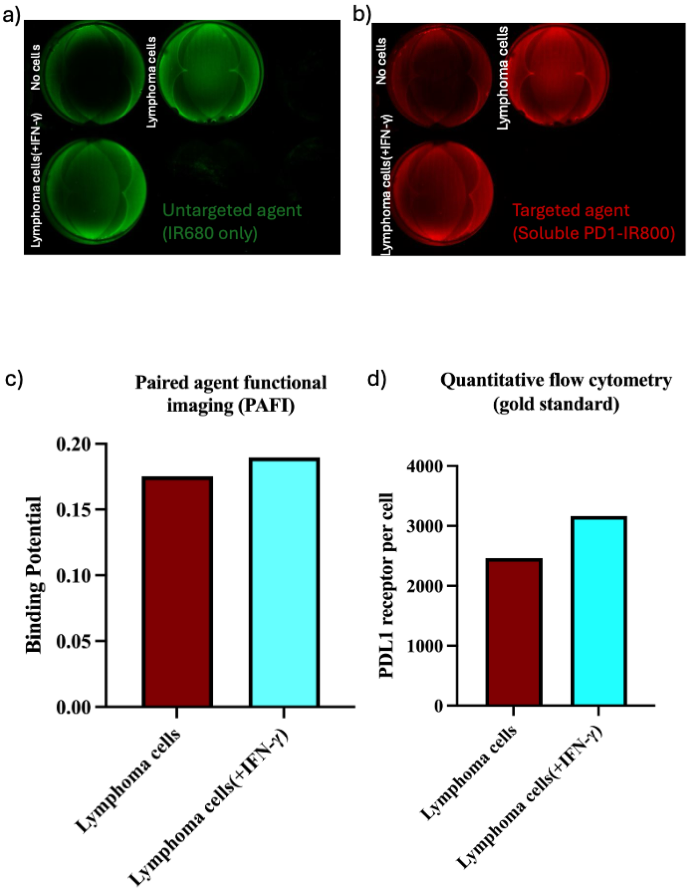
\includegraphics[width=\linewidth]{Thesis Template - LaTeX/figures/tissue-cells.png}

        % Phantom labels for subfigure referencing
        \begin{minipage}{0pt}
            \phantomsubcaption\label{fig:tissue-cells_a}
            \phantomsubcaption\label{fig:tissue-cells_b}
        \end{minipage}

        \captionsetup{justification=raggedright, singlelinecheck=false}
        \caption[Binding Potential-Total receptor comparison]{\textbf{PAFI quantifies functional PDL1 in lymphoma models.}
        (a) Representative images of untargeted and (b) targeted agent signals in tissue-mimicking phantoms with no cells, lymphoma cells, and IFN-$\gamma$–treated lymphoma cells after imaging. (c) Bar graphs comparing BP to (d) total PDL1 expression measured by QFC.}
        \label{fig:tissue-cells}
    \end{minipage}
\end{figure}

\begin{figure}[H]
    \centering
    \begin{minipage}{1\linewidth}
        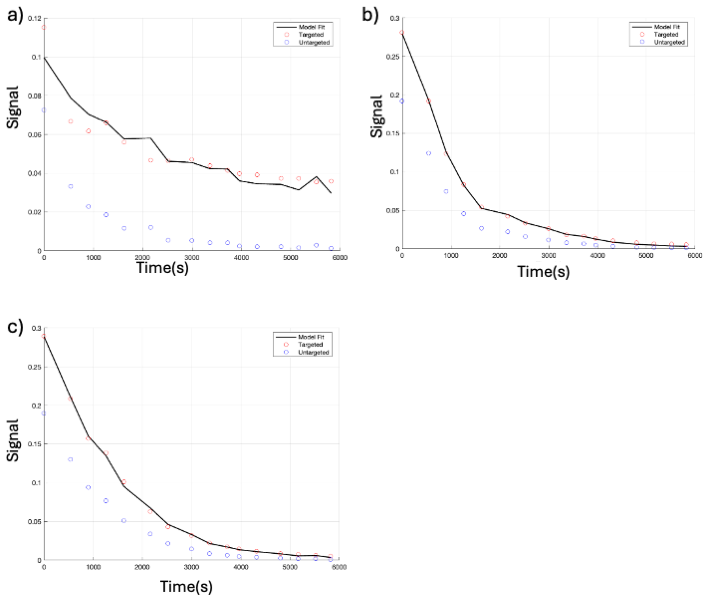
\includegraphics[width=\linewidth]{Thesis Template - LaTeX/figures/bp_plots.png}
        \captionsetup{justification=raggedright, singlelinecheck=false}
        \caption[Binding potential fits]{
            \textbf{Combination fluorophore experiments set up.} 
            (a) Control condition (no cells), (b) IFN-$\gamma$–treated lymphoma cells, and (c) untreated  Lymphoma cells. In each panel, red circles represent the signal from the targeted agent (PD1-IR800), blue circles indicate the untargeted agent (IR680), and the black line represents the model fit used to calculate binding potential (BP). The calculated BP values were 2.342 for the control, 0.1898 for the IFN-$\gamma$–treated condition, and 0.1753 for the untreated condition.
        }
        \label{fig:bp_plots}
    \end{minipage}
\end{figure}
